\section{Resource Development and Reconstruction} \label{sec:develop}
The general workflow of DOREMUS is depicted in Fig.~\ref{fig:doremus}. The data from the three partner institutions is first converted to RDF following the DOREMUS model, resulting in three independent knowledge graphs (one per institution), which are then linked. After a manual validation of a set of uncertain links, a pivot graph is built containing identifiers of the union of all works found in the three graphs, together with identity links to the resources in each of the three institutional graphs. We detail on these stages of the workflow in this section. 

%\vspace{-2cm}

\subsection{Data Conversion}
The data collected from the BnF and the PP describing music works is represented in the UNI-- and INTERMARC variants of the MARC format. A MARC file is a succession of fields, each carrying a 3-digit label, and subfields, delimited by the \$ symbol (e.g., ``50011\$313908188\$qSonates\$rPiano\$sOp.27, no 2\$uDo   mineur").\footnote{For detailed information, we refer to the documentation released by The International Federation of Library Associations and Institutions (IFLA){\url{http://www.ifla.org/publications/ifla-series-on-bibliographic-control-36}}}. We have developed an open source prototype, named {\tt marc2rdf} to automatically convert UNI- or INTERMARC bibliographic records to RDF, implementing the DOREMUS model (link to the tool given in Table \ref{tab:links}). The conversion process relies on explicit expert-defined transfer rules (or mappings), which provide the corresponding property path in the model as well as useful examples \cite{lisena2016exploring}. We have used the DOREMUS properties to name the extracted relations (e.g., \texttt{mus:U12$\_$has$\_$genre} is the property describing the genre of a work). Beyond being a  documentation for the MARC records, these rules embed  information on specific and distinct librarian practices in the formalization of the content (format of dates, syntax of textual fields, default values for missing information), making \texttt{marc2rdf} a robust generic converter for MARC files.

\begin{figure}[t]
\center
	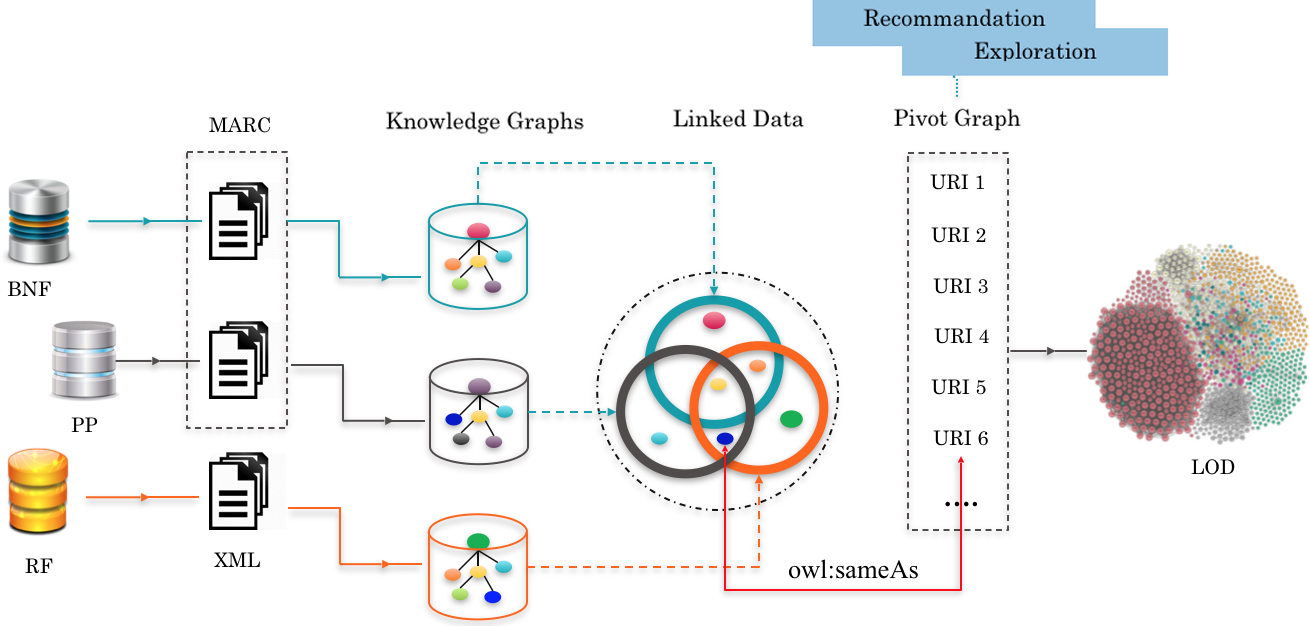
\includegraphics[width=11cm]{img/DRMS-WRKFL.png}
	\caption{The DOREMUS data lifecycle.}
	\label{fig:doremus}
%\end{figure}
\smallskip
%\begin{figure}
  \centering
  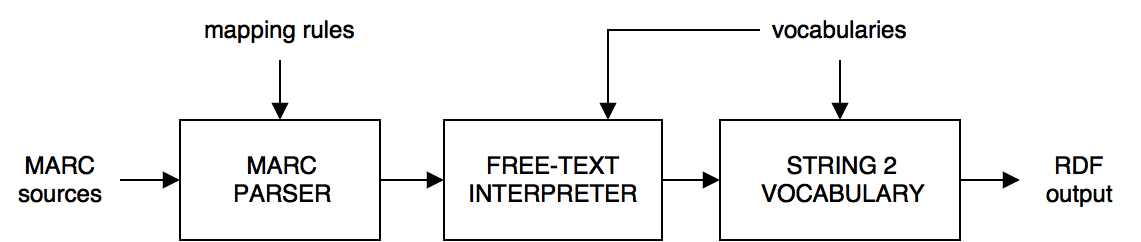
\includegraphics[width=8.5cm]{img/marc2rdf_schema.png}
  \caption{The application flow of \texttt{marc2rdf}.}
  \label{fig:marc2rdf}
\end{figure}

The converter is composed of different modules that work in succession (Fig.~\ref{fig:marc2rdf}). First, a \textit{file parser} reads the MARC file and makes the content accessible by field and subfield number. We implemented a converting module for both the INTERMARC and UNIMARC variants. Then, it builds the RDF graph reading the fields and assigning their content to the DOREMUS property suggested in the transfer rules. The \textit{free-text interpreter} extracts further information from the plain text fields, that includes editorial notes. This amounts to do a knowledge-aware parsing, since we search in the string exactly the information we want to instantiate from the model (i.e., the MoP from the casting notes, or the date and the publisher from the first publication note). The parsing is realized through empirically defined regular expressions, that are going to be supported by Named Entity Recognition techniques as future work. Finally, the \textit{string2vocabulary} component performs an automatic mapping of string literals to URIs coming from controlled vocabularies. All variants for a concept label are considered in order to deal with potential differences in naming terms. As additional feature, this component is able to recognize and correct noise that is present in the MARC file: this is the case of musical keys declared as genre, or fields for the opus number that actually contain a catalog number and vice-versa.

The {\tt marc2rdf} tool allows to reproduce deterministically the conversion process at any moment in time, providing the opportunity to seamlessly take into account possible updates of the ontology (e.g., the addition of a new property) and/or the data entries (a new record entering the catalog of one of the institutions), ensuring in that way the currentness and dynamics of the graphs. 

The works from Radio France, described in XML, are managed by an \textit{ad hoc} software that parses the input file, collects the required information, creates the RDF graph structure  and runs the \textit{string2vocabulary} module.% described previously.%\todo{I'm aware of the problem, but not providing a link to the converter might compromise the paper. Any ideas of solution?}

\subsection{Data Linking}
The three datasets that are currently subject to interlinking are highly heterogeneous: a given entity (e.g., a musical work) can be described quite differently across the three institutions. In addition to well-known data discrepancies such as lexical, semantic (polysemy, synonymy) and orthographic mismatches of string literals, the use of acronyms and abbreviations or differences in formats and types of numerical values, we have encountered several commonly occurring issues that are specific to our data. We outline some of them below.

%\begin{enumerate}
---~{\it Differences in coverage} and particularly lack of information in one of the graphs as compared to a richer description in another. In our case, the  works coming from RF are systematically described by a considerably smaller set of attributes, than those found in the catalogs of the BnF and the PP (see Table~\ref{tab:stats}). 

--- {\it Different depths in the graphs}, at which we find the value of interest---e.g., the birthplace of a composer can be directly assigned to the entity in one graph, or via a longer property chain in another. 

--- Presence of {\it comments in the form of free text} (given by the property {\tt ecrm:P3\_has\_note}) that are difficult to compare, as well as presence of {\it institution-specific resource identifiers} (bibliographical records ID's) given under the same property name across different datasets, although not comparable.% and therefore of little use for the linking task.

--- Presence of {\it blocks of  highly similar in their descriptions, but yet distinct instances} in each of the graphs---e.g., the set of all piano sonatas by Beethoven, differing from one another in only one or two property values, which makes their disambiguation difficult and is likely to produce false positives. 
%\end{enumerate}

In a first attempt to interconnect these graphs, we relied on state-of-the-art linking systems \cite{jentzsch2010silk,ngomo2011limes} that adopt a property-based philosophy where a set of attributes is selected in order to compare instances across two datasets based on (an aggregation of) similarity measures computed on their literal values. The results obtained proved to be not satisfactory.\footnote{Evaluation results of {\it Legato} on OAEI benchmarks can be found at \url{https://github.com/DOREMUS-ANR/legato/blob/master/Legato-Results.png}. Data and configuration files for SILK are available at \url{https://github.com/manoach/SILK-Evaluation}. Note that SILK is configured by using the best keys selected by the algorithm in \cite{achichiEST16}.}. Consequently, we develop our own linking tool, named \textit{Legato} \cite{achichi2017legato}---a generic data linking system motivated by the DOREMUS use-case scenario and data linking challenges. 

\begin{figure} 
\center
	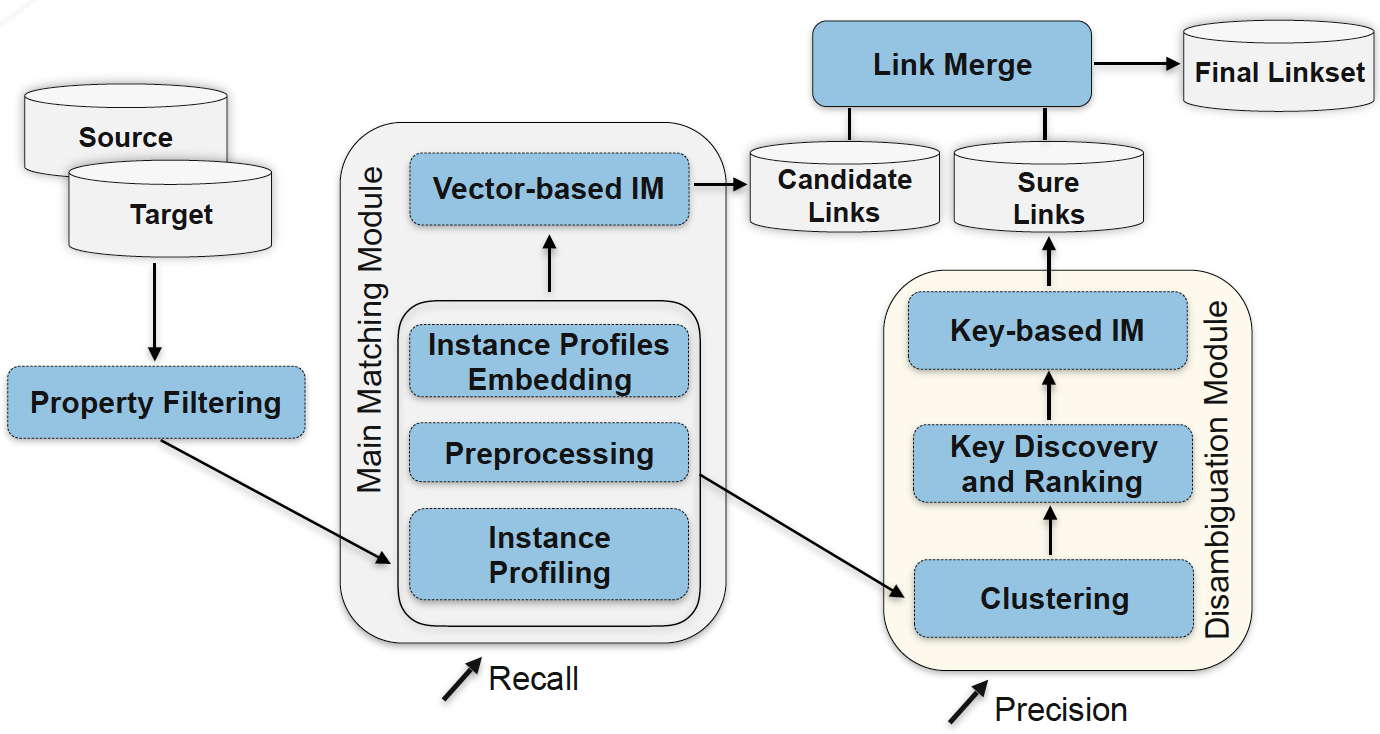
\includegraphics[width=9cm]{img/legato-wf-3.png}
    %\vspace{-0.2em}
	\caption{Processing pipeline of \textit{Legato}.}
	\label{fig:workflow}
	%\vspace{-2.5em}
\end{figure}

{\it Legato} is designed to match entities from highly heterogeneous graphs, effectively disambiguating highly similar yet distinct resources. Fig.~\ref{fig:workflow} shows the generic workflow of the system. The data cleaning module ensures to only keep properties that are comparable across the datasets (hence, comments in the form of free text, as well as institution-specific instance identifiers are removed). The instance profiling module represents instances by a subgraph corresponding to the union of the Concise Bounded Descriptions (CBD)\footnote{\url{https://www.w3.org/Submission/CBD/}} of each resource and its direct neighbors.  In that, contrarily to SILK or Limes, Legato (in its default version) does not compare property values, but considers all extractable literal values as a bag-of-words.  This representation addresses in its mechanism a number of data heterogeneities without requiring user input, in particular, the description differences and property depths discrepancies outlined above. The literals of these subgraphs are then used to project each instance in a vector space and the matching consists in comparing the resulting vectors. A deliberately low threshold is used for the vector similarity in order to ensure  high recall. Then, highly similar instances are grouped together by the help of a standard hierarchical clustering algorithm~\cite{RokachM05a}. An RDF key discovery \cite{SAKey} and a key ranking \cite{achichiEST16} algorithms are applied on each pair of similar clusters (identified by comparing cluster centroids) across the two graphs, in order to identify the set of properties that best allow to discriminate between the resources contained in each cluster. A new linkset (called ``sure links") results from this process and is then compared to the links produced at the matching step (called ``candidate links") in order to eliminate errors and increase precision, leading to the production of the final linkset. The outcome of {\it Legato} is presented in the EDOAL format,\footnote{\url{http://alignapi.gforge.inria.fr/edoal.html}}  allowing to keep track of the associated confidence scores, or as {\tt owl:sameAs} triples. We provide an open source implementation of the system together with a simple user interface (see Table \ref{tab:links} for a link).

Given our knowledge of the DOREMUS data, we have customized the linking process for the purposes of the project in two respects. (1) The linking workflow begins by searching for values of the composer name and catalog number properties, because the set of these two properties has been identified as a key by our experts. If values for these two properties are found for a given pair of instances, they are directly used for the comparison and {\it Legato} is executed on the remaining instances only. Note, however, that these properties do not have values for a very large number of works and in particular, no entry of {\tt itema3} has a catalog number (cf. Table~\ref{tab:stats}). (2) In order to speed-up the execution of {\it Legato}, we have partitioned the datasets per composer and linked pairs of subsets across two graphs that gather works by the same composer.

To evaluate {\it Legato}, we have constructed benchmarks of music works from the BnF and the PP, by asking the librarian experts to manually select pairs of identical resources from the their respective catalogs. We have ensured that our benchmarks are representative and provide a fair account of the heterogeneity issues outlined above. This results in the generation of two  benchmarks  that have been released by the Instance Matching track of OAEI 2016 and 2017 (cf. Table \ref{tab:links}). {\it Legato} has participated to the 2017 edition of the campaign, ranking first on the DOREMUS-FPT task. NjuLink surpasses {\it Legato} by 0.025 points (F1) on the DOREMUS-HT track, but performs worse by 0.044 points on the FPT track. Our data exhibits characteristics of the two, therefore we decided to go for {\it Legato}, in addition to the customizability argument given above.  
%(results are available on the OAEI 2017 website).

\subsection{ Link Validation and Pivot Graph Construction} \label{sec:pivot}
As a result of the pair-wise alignments of the three graphs, we end up with three sets of links. We exploit the topology of the connectivity of the entities of the three graphs in order to define subsets of links to provide to data experts for manual validation, aiming to ensure a final set of links of high quality. We identify four connectivity patterns, shown in Fig.~\ref{fig:cases}, according to which we classify the produced links to three categories: {\it certain links}, {\it invalid links} and {\it validation candidates}. The classification of a link as ``certain" depends both on its confidence value and on the connectivity pattern in which it falls. The certain links are retained and included in the pivot graph constructed from our data (see below). If a link is approved by an expert during the user validation process, its confidence value is set to 1, which automatically classifies it as ``certain", else it is declared as ``invalid". We consider the following link patterns.

\begin{figure} 
\center
	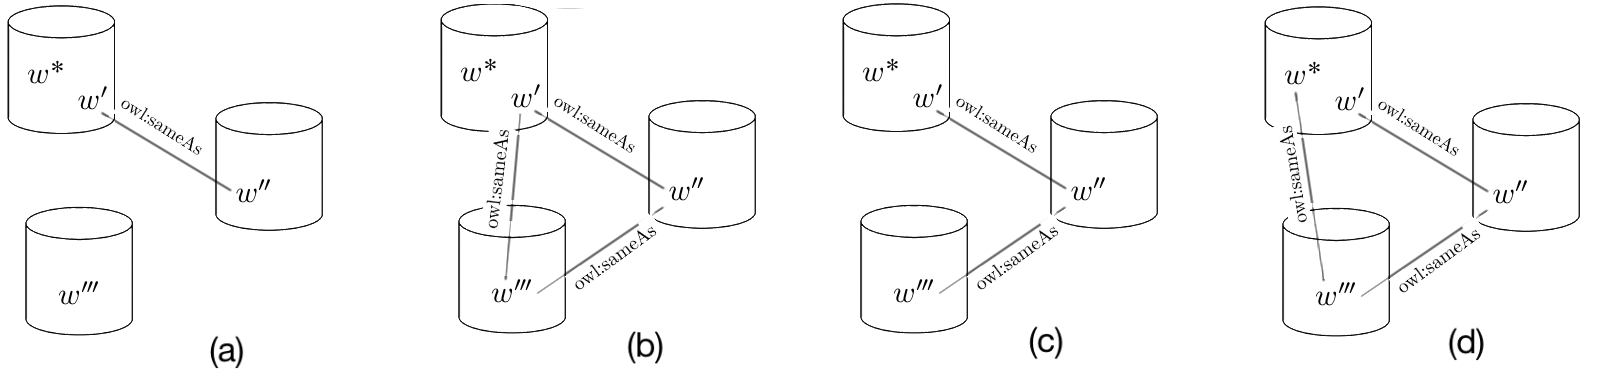
\includegraphics[width=12cm]{img/links-cases.png}
    %\vspace{-0.2em}
	\caption{Links across the three graphs: four connectivity patterns.}
	\label{fig:cases}
	%\vspace{-2.5em}
\end{figure}

%\begin{enumerate}
%\item 
(1) Single link. This is the case when two works are connected via an identity link across their corresponding graphs as a result of the automatic linking process (Fig.~\ref{fig:cases}(a)). According to the confidence value of the link, it is either classified as  certain, passed over to the experts for validation, or discarded.

(2) Triangle. This is the case when three works from the three graphs are linked via three {\tt owl:sameAs} relations. In this case, the three links are considered as certain and the expert is not solicited (Fig.~\ref{fig:cases}(b)).

(3) Missing link. This is the case when an instance $w'$ from one graph is linked to an instance $w''$ from the second graph, which in turn is linked to an instance $w'''$ from the third graph, but no link has been created between $w'''$ and $w'$ (Fig.~\ref{fig:cases}(c)). Instead of inferring that link, independently on the links confidence values, we pass the two link candidates $<w'$, {\tt owl:sameAs}, $w'' >$, $<w''$, {\tt owl:sameAs} $w'''>$ to the experts for validation. If the validation process results in classifying these two links as certain, the link $<w'''$, {\tt owl:sameAs}, $w'>$ is inferred and classified as certain. Note that the third link inference mechanism is activated only in case we have two certain links.

(4) Conflict. This is the case when an instance $w'$ from one graph is linked to an instance $w''$ from the second graph, which in turn is linked to an instance $w'''$ from the third graph, and $w'''$ is linked to an instance $w^*$ from the first graph, where $w' \neq w^*$  (Fig.~\ref{fig:cases}(d)). All three links are passed to the experts for validation. This necessarily leads to invalidating at least one of the three links, in which we fall into one of the three cases described above.
%\end{enumerate}

\begin{figure} 
\center
	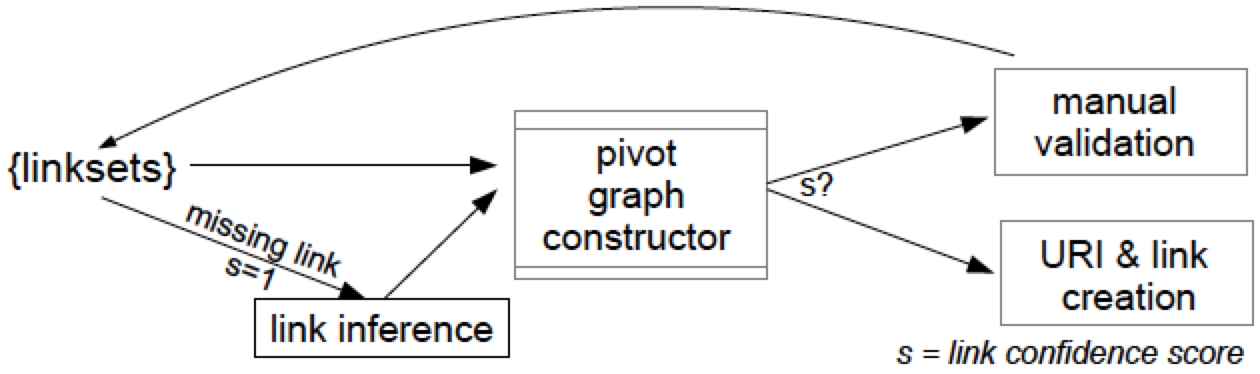
\includegraphics[width=7cm]{img/pivot-graph-2.png}
    %\vspace{-0.2em}
	\caption{Link validation and pivot graph construction workflow.}
	\label{fig:pivot}
\end{figure}

\vspace{-0.8cm}

\paragraph{Pivot Graph Construction.}
We construct a referential pivot graph of music works that is the mathematical union of the three sets of works from the three partner institutions. As an editorial decision, a novel URI is created for every entity in that graph, following the URI creation pattern described previously, together with a {\tt owl:sameAs} link to the URIs identifying this entity in each of the three input graphs (at least one such URI exists). For example, if a given expression is described in both the BnF and the PP graphs, the pivot graph will contain the following two triples: 
$<$PIVOT\_URI$>$ {\tt owl:sameAs} $<$BNF\_URI$>$, $<$PP\_URI$>$. If the work exists  in one single graph only (e.g., the  one of BnF), one single triple will be declared: $<$PIVOT\_URI$>$ {\tt owl:sameAs} $<$BNF\_URI$>$. To reconstitute these links, we rely on the linksets produced in the data linking phase and on the manual link validation task. As explained above, as a result of these processes, we end up with three sets of ``certain" links. Only links from that category will appear in the pivot graph. As Fig.~\ref{fig:pivot} shows, the process of pivot graph construction and that of the manual validation of links are tangled up in a single workflow. The code of the algorithm for (re-)generating the pivot graph is released as open source (cf. Table \ref{tab:links}).

Currently, the manual validation process is in progress. Therefore, the published pivot graph contains the links that have been identified automatically (i.e., corresponding to the patterns in Figs.~\ref{fig:cases}(a) and~\ref{fig:cases}(b)) by using the non-conservative thresholds of {\it Legato} tuned by the help of our benchmarks (0.2 for {\tt bnf}-{\tt philharmonie} and 0.5 for the other two pairs of datasets). The graph contains also the links of all unique works (those that have no matches found in any of the two other bases) to their original URIs. The results of the automatic link discovery process on the three bases together with the resulting pivot graph in its current shape are available at \url{https://github.com/DOREMUS-ANR/knowledge-base/tree/master/linked-data}. 

\paragraph{Links statistics.}

We have currently a total of 7495 links created automatically across the three graphs, among which we have 2520 links of type {\it single link}, 396 links of type {\it triangle}, 3378 links  of type {\it missing link} and 261 links  of type {\it conflict} (as labeled in Fig.~~\ref{fig:cases}), plus additional 940 links of type 1:many that are currently subject to post-processing. Updates in the datasets will not decrease the number of links since the source databases monotonically grow. 

%We have currently a total of 107684 links created automatically across the three graphs, among which we have 2887 links of type {\it single link}, 68886 links of type {\it triangle}, 2174 links  of type {\it missing link} and 293 links  of type {\it conflict} (as labeled above and illustrated in Fig.~~\ref{fig:cases}). Currently, this makes a total of 2467 links to validate manually, or $3\%$ of the total number of links produced. However, this number can potentially increase if more conservative thresholds are selected for the manual validation. Updates in the datasets will not decrease the number of links since the source databases monotonically grow. 
